This section will apply the results in Section \ref{sec:useful} about useful components to
deterministic matched subspace detection. In this detection setting, we are given a high
dimensional test observation and wish to discriminate between the $H_0$ hypothesis that
the observation is purely noise and the $H_1$ hypothesis that the observation contains a
low-rank-$k$ signal that lies at a fixed point in an unknown subspace. To design a
detector, we have access to a training dataset of signal bearing observations.
We assume that the training data was collected in a variety of representative experimental
conditions, allowing each observation's signal component to lie at a different location in
the signal subspace. This setup is the similar to that in \cite{asendorf2013performance}
and the resulting standard matched subspace detector is an energy detector with the same
form as (\ref{eq:the_detector}). We use random matrix theory to determine the number of
informative subspace components, $\keff$, which is an upper bound for
$\kuse$. Through a numerical example, we demonstrate the relationship between the standard
plug-in detector using exactly $k$ subspace components, a detector using $\keff$ subspace
components, and a detector using exactly $\kuse$ subspace components.

\subsection{Training Data Model}\label{sec:training_data}

Let $U=[u_1,\dots,u_k]\in\reals^{n\times k}$ be an unknown signal subspace matrix with
pairwise orthonormal columns $u_i\in\reals^{n\times 1}$. To estimate $U$, 
we are provided a dataset containing $m$ signal-bearing training vectors
$y_i\in\reals^{n\times 1}$, $i=1,\dots,m$, modeled as 
\beq\label{eq:taes_train}
y_i=Ux_i+z_i 
\eeq 
where
$z_i\overset{\text{i.i.d.}}{\sim}\mathcal{N}(0,I_n)$ and
$x_i\overset{\text{i.i.d.}}{\sim}\mathcal{N}(0,\Sigma)$ where
$\Sigma=\diag(\sigma_1^2,\dots,\sigma_k^2)\in\reals^{k\times k}$ with
$\sigma_1>\sigma_2>\dots>\sigma_k>0$ known. For each observation, $x_i$ and $z_i$ are
independent. In the training data, $x_i$ is modeled stochastically to represent the
variety of conditions under which the training data may be collected.  We assume that the
dimension, $k$, of our subspace is known and that $k\ll n$ so that we have a low-rank
signal embedded in a high-dimensional observation vector. Applications in which training
datasets arise include MIMO radar \cite{chen2013adaptive}, GNSS receivers
\cite{arribas2013antenna}, source localization \cite{he2013near}, DOA
\cite{liao2013direction}, and target detection \cite{kwon2013multi}. In such applications,
we may think of the entries of $y_i$ received data from an antenna array, $U$ as the
channel response matrix, $x_i$ as the transmitted waveform, $\Sigma$ as the signal-to-noise
ratio (SNR) matrix, and $z_i$ as additive noise.

\subsection{Testing Data Model}

In the testing setting, we are given an unlabeled observation $y\in\reals^{n\times 1}$
modeled as
\begin{equation}\label{eq:determ_setup}
y=\left\{
\begin{aligned}
&z
&& y\in H_0:\text{ Noise only}\\
&U\Sigma^{1/2} x+z
&& y\in H_1:\text{ Signal-plus noise}\\
\end{aligned}\right. ,
\end{equation}
where $U$, $\Sigma$, and $z$ are modeled the same as the training data as described in
Section \ref{sec:training_data}. However, for the test observations, $x=[x_1,\dots,x_k]^T$
is a non-random, unknown deterministic vector. Thus the signal, $U\Sigma^{1/2}x$, lies at a
fixed point in the unknown subspace. Note that $\Sigma$ controls the SNR of each subspace
component.

\subsection{Subspace Estimation and Accuracy}\label{sec:param_estim}

In the testing model, the signal subspace $U$ is unknown and must be estimated from the
provided training data. Given the signal bearing training data 
\be
Y = \left[ y_1, \dots, y_m \right]\in\reals^{n\times m},
\ee 
we form the sample covariance matrix
$S=\frac{1}{m}YY^{T}$. The covariance matrix of a training observation is $\E{y_iy_i^T} = U\Sigma
U^T +I_n$ and it follows that the (classical) maximum likelihood estimates (in the many-sample, small
matrix setting) for $U$ is given by 
\beq\label{eq:param_estims_stoch}
\widehat{U}=[\widehat{u}_1 \dots \widehat{u}_{k}] \eeq
where
$\widehat{u}_1,\dots,\widehat{u}_{k}$ are the eigenvectors of $S$ corresponding to the
largest $k$ eigenvalues \cite{muirhead1982aspects} .

In any real world setting, we have finite training data and finite SNR. Therefore,
$\widehat{U}$ is inaccurate and degrades the performance of any detector that relies on it.
Proposition 5.1 of \cite{asendorf2013performance}  characterized the asymptotic accuracy of the
eigenvectors of the sample covariance matrix $S$ stating that as $n,m\to\infty$ with $c=n/m$
\beq\label{eq:angles}
|\langle u_i,\widehat{u}_i\rangle|^2 \convas
\begin{cases}
\dfrac{\sigma_i^4-c}{\sigma_{i}^4+\sigma_{i}^2c} & \text{ if } \sigma_{i}^2>\sqrt{c}\\
0 & \textrm{otherwise}\\
\end{cases}.  \eeq We note that $\convas$ denotes almost sure convergence. The key insight
to (\ref{eq:angles}) is that only the eigenvectors corresponding to the signal variances,
$\sigma_i^2$, lying above the phase transition $\sqrt{c}$ are
\textit{informative}. Following \cite{asendorf2013performance, nadakuditi2008sample}, we
define the effective number of (asymptotically) identifiable subspace components
$k_\text{eff}$ as:
\begin{equation}\label{eq:keff}
k_\text{eff} = \text{Number of } \sigma_i^2 > \sqrt{c}.
\end{equation}

\subsection{Plug-in and RMT Detectors}

If $U$ was known, the matched subspace detector is the GLRT using the test statistic (see
\cite{scharf1994matched,vincent2008matched,fuchs2007robust})
\be
\Lambda(w) = y^TUU^Ty = w^Tw
\ee
where $w=U^Ty\in\reals^{k\times 1}$. This is clearly an energy detector of the same form as
(\ref{eq:the_detector}) where each component of $w$ is the energy of $y$ residing in that
direction of the subspace. However, this detector is not realizable as $U$ is unknown and
so we substitute $\widehat{U}$ for the unknown $U$, resulting in the plug-in detector
\cite{asendorf2013performance}
\beq\label{eq:plugin_stat}
\Lambda_{\text{plugin}}(\widehat{w})= \widehat{w}^T\widehat{w} = \sum_{i=1}^k \widehat{w}_i^2
\eeq 
where $\widehat{w} = \widehat{U}^T y$ is the projection of the test observation onto the
estimated subspace. Similar plug-in techniques using sample covariance matrices occur in
direction detection \cite{santiago2013noise} and GNSS receivers \cite{arribas2013antenna}. The plug-in detector incorrectly assumes that $\widehat{U}=U$ and consequently
that all $k$ subspace components are informative. To avoid some of the performance loss of the
plug-in detector associated with including uninformative subspace components, we derived a
RMT detector that only includes the informative subspace components (see \cite{asendorf2013performance} for a derivation). The
RMT detector statistic is 
\beq\label{eq:rmt_stat}
\Lambda_{\text{rmt}}(\widehat{w})= \sum_{i=1}^{\keff}\widehat{w}_i^2.
\eeq

Clearly, both the plug-in and RMT detectors are energy detectors of the form in 
(\ref{eq:the_detector}) and so we may use (\ref{eq:roc_energy}) to analyze the performance
of each detector. In the MSD application, $\delta_i = \sigma_i|\langle
u_i,\widehat{u}_i\rangle| s_i x_i$ where $s_i\in\left\{1,-1\right\}$ represents the
random phase ambiguity in the eigenvector computation. Therefore, the non-centrality
parameter for this problem is 
\beq\label{eq:msd_nc_param}
\lambda_d = \sum_{i=1}^d \sigma_i^2|\langle u_i,\widehat{u}_i\rangle|^2x_i^2
\eeq
where the plug-in detector uses $d=k$ subspace components and the RMT detector uses
$d=\keff$ subspace components. In \cite{asendorf2013performance}, we demonstrated that the
plug-in detector is suboptimal and that the RMT detector will always achieve the same or
better performance.

\subsection{Relationship between $\kuse$ and $\keff$}

We first note that $\kuse\leq\keff$. If a subspace component is uninformative ($|\langle
u_i,\widehat{u}_i\rangle|^2 =0$ as determined by (\ref{eq:keff})), that component
contributes nothing to the non-centrality parameter as defined in
(\ref{eq:msd_nc_param}). From the analysis in Section \ref{sec:useful}, including this
subspace component in a detector would degrade detector performance. Therefore, a subspace
component must be informative to be one of the $\kuse$ subspace components. 

However, the number of useful subspace components may be strictly less than the number of
informative subspace components. As demonstrated in Figure \ref{fig:nc_lines}, when adding
an additional subspace component, the increase in non-centrality parameter must exceed a
minimum value. Examining (\ref{eq:msd_nc_param}), the non-centrality parameter depends on
$\Sigma$, $x$, and the accuracy of the eigenvectors of the sample covariance matrix
($|\langle u_i, \widehat{u}_i\rangle|^2$). Depending on these values, adding the $i$-th
component may not increase the non-centrality parameter enough to improve detection, even
when the subspace component is informative ($|\langle u_i,
\widehat{u}_i\rangle|^2>0$). Thus, it is possible for informative subspace components to
not be useful in detection.

Besides the desired false alarm rate, $P_F$, $\kuse$ also depends on $\Sigma$ and $x$ for
the matched subspace detector. Larger values of $|x_i|$ and $\sigma_i$ lead to larger
non-centrality parameters as defined in (\ref{eq:msd_nc_param}), making it more likely for
that component to be useful.  This is intuitive because the larger $|x_i|$ and $\sigma_i$
force the mean of the conditional distribution of $\widehat{w}_i|H_1$ further from 0,
which is the mean of the conditional distribution of $\widehat{w}_i|H_0$.  If we
instead fix $\Sigma$, $n$ , and $x$ and allow $m$ to change, we observe that more training
data increases the accuracy the subspace estimate as seen in (\ref{eq:keff}). Therefore,
increasing $m$ increases $\delta_i$, which may make subspace components useful.

The number of informative subspace components, $\keff$, is an upper bound for the number
of useful subspace components, $\kuse$. As mentioned earlier, we cannot compute $\kuse$ in
closed form because the deterministic vector $x$, which drives the non-centrality
parameters $\delta_i$, is unknown. Therefore, $\kuse$ is an oracle statistic as so we use
$\keff$ as a proxy for $\kuse$ in a realizable detector. However, as $\keff$ does not depend
on $x$, whenever $\keff\neq\kuse$, detectors using $\keff$ subspace components will be
suboptimal.

Finally, we note that the derivation and computation of $\kuse$ for the matched subspace
detection application relies on random matrix theory. Without these insights, we would
have no expression for $|\langle u_i,\widehat{u}_i\rangle|^2$ and subsequently could not
compute the non-centrality parameter in (\ref{eq:msd_nc_param}) to use in the algorithm in
Figure \ref{algo:kuse}.

\subsection{Numerical Example}

In Figure \ref{fig:main_result} we compare the performance of the plug-in and RMT
detectors to the performance of a detector that uses $d=\kuse$ subspace components. We
consider the setting when $k=3$, $n=200$, $\Sigma=\diag(5,2,0.5)$, and
$x=[1.5,1.5,1.5]^T$. For a fixed $P_F=0.1$, Figure \ref{fig:det_perf} plots the
theoretical detection probability (as computed in (\ref{eq:roc_energy}) using
(\ref{eq:keff}) and (\ref{eq:msd_nc_param})) given various amounts of training
data. Results are shown for the plug-in ($d=k$), RMT ($d=\keff$), and useful ($d=\kuse$)
detectors. Figure \ref{fig:dvals} plots the
corresponding number of subspace components each uses given various amounts of training
data.

\begin{figure}[t]
\centering
\subfigure[Detector Performance]{
  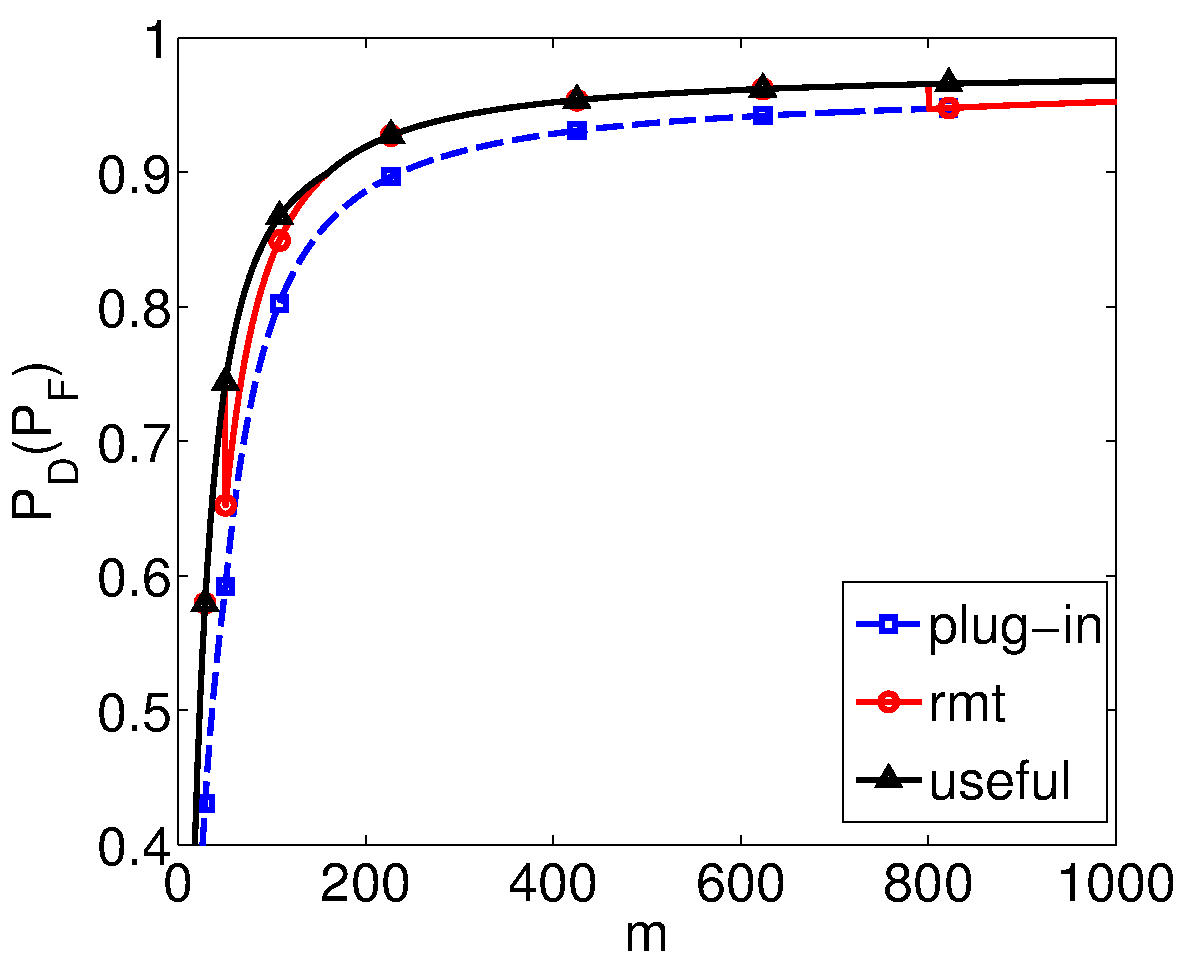
\includegraphics[width=0.45\textwidth]{taes_msd/figures/taes_pd_v_m.pdf}
  \label{fig:det_perf}}
\subfigure[Number of Subspace Components]{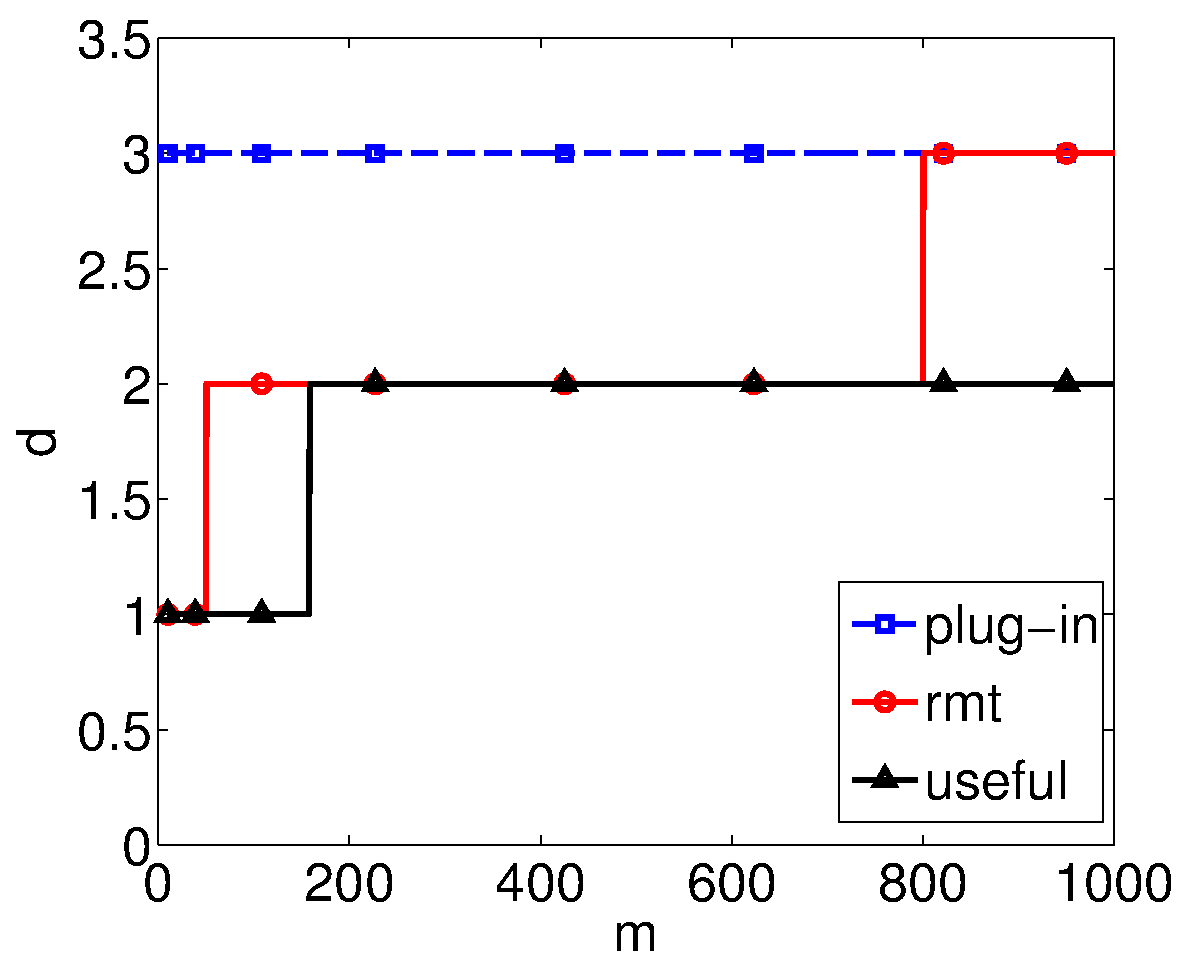
\includegraphics[width=0.45\textwidth]{taes_msd/figures/taes_d_v_m.pdf}
  \label{fig:dvals}}
\caption{Deterministic energy detector performance as a function of the number of training
  samples. In this experiment $n=200$, $\Sigma =\diag(5,2,0.5)$, $x=[1.5,1.5,1.5]^T$, and
  the required false alarm rate is $P_F=0.1$. (a) The theoretical probability of detection
  achieved by the plug-in, RMT, and useful detectors. $P_D(P_F)$ is calculated in
  (\ref{eq:roc}). The plug-in detector sets $d=k$, the RMT detector sets $k=\keff$ as
  defined in (\ref{eq:keff}), and the useful detector sets $d=\kuse$ as calculated in
  Figure \ref{algo:kuse} using the non-centrality parameter defined in
  (\ref{eq:msd_nc_param}). The useful detector achieves the optimal performance. (b) The
  number of subspace components used by the plug-in, RMT, and useful detectors. Whenever
  $\keff\neq\kuse$, the RMT detector realizes a suboptimal detector performance. Even
  though these subspace components are \textit{informative}, there is not enough training
  data to make them \textit{useful} in detection.}
\label{fig:main_result}
\end{figure}

Evident in Figure \ref{fig:det_perf}, the detector using $\kuse$ subspace components
achieves the maximum detection ability of all detectors for every amount of training
samples. This is slightly contrived because $\kuse$ is optimized to do just this. More
importantly, we empirically see that using $\keff$ subspace components is not always
optimal.  However, examination of Figure \ref{fig:dvals} reveals why this occurs. For
$50\leq m\leq 160$, $\keff=2>\kuse=1$. Therefore, even though the second subspace
component is informative by definition, it is not \textit{useful} in detection. Including
it in an energy detector decreases detector performance. A similar phenomenon
occurs at $m=800$ when $\keff$ increases to 3 but $\kuse$ remains constant at 2. Unlike
the RMT detector, the detection performance of the useful detector increases monotonically
with an increase in training samples. Both the RMT and useful detectors outperform the
standard plug-in detector which uses all $k$ subspace components.
